\chapter{Introduction}

% - Early geodesy
% - long sampling rates
% - cannot resolve time dependence

Since the seminal report by \citet{Reid1910}, it has been recognized
that earthquakes are caused by the sudden release of elastic strain
energy that has gradually accumulated over time along faults. This is
known as elastic rebound theory. \citet{Reid1910} introduced elastic
rebound theory to explain ground deformation leading up to and as a
result of the 1906 San Francisco earthquake. In the report,
triangulation surveys showed that the ground on either side of the San
Andreas fault and at far distances from the fault was steadily
undergoing a shearing motion at a rate of about 6 cm/year. During the
1906 earthquake, the San Andreas fault slipped by about 6 meters,
presumably releasing the elastic strain energy in the crust that has
accumulated over the past hundred years or so. Modern geodetic
techniques have updated the rate of deformation across the San Andreas
fault to about 3 cm/year \citep{Savage1973}, but elastic rebound
theory has remained generally accepted since its inception over a
century ago.

Elastic rebound theory forms the foundation of seismic hazard models
such as the third Unified California Earthquake Rupture Forcast
(UCERF3) \citep{Field2014}. Geodetic observations can tell us the rate
that strain is accumulating between tectonic plates. Based on elastic
rebound theory, this built up strain will inevitably be relaxed through
fault slip. It is then possible to use geodetic data to estimate the
long term fault slip rates that are needed to accomodate tectoncially
accumulated strain \citep[e.g.,][]{Savage1973,Meade2005}. UCERF3 uses
geodetically and geologically derived slip rates for the San Andreas
Fault system in conjunction with various other assumptions to estimate
the likelihood that a major earthquake would occur over some window of
time in California. UCERF3 has clear societal implications; it is used
by engineers for designing buildings, and it is used by the California
Earthquake Authority for determining earthquake insurance rates.

In constraining UCERF3, it is assumed that strain is building up on
the San Andreas Fault system at a constant rate over time. However,
time-dependent, or transient, deformation around fault zones is a
frequently observed phenomena that casts doubt into this assumption
\citep{Thatcher1983}. By better understanding transient deformation
and the mechanisms causing it, we can then conceivably improve upon
existing seismic hazard models. Some of the earlier records of
transient deformation came from repeated leveling or triangulation
surveys made after large earthquakes \citep[e.g.,][]{Tsuboi1932,
Smith1968}. These studies revealed elevated rates of ground
deformation following the earthquakes, which then decayed over a
timescale of months to years. This type of transient deformation is
referred to as postseismic deformation.

Over the past few decades, Global Navigation Satellite Systems
(GNSS)\footnote{The terms ``GNSS" and ``GPS" (Global Positioning
System) will be used synonymously in this dissertation, although GPS
is specifically operated by the United States and GNSS is a more
generic term.} have become a valuable geodetic tool for observing
transient deformation. Throughout most of the 20th century, geodetic
techniques, such as triangulation and leveling surveys, required
someone to be physically present at the geodetic monuments in order to
make an observation. Consequently, the time interval between
consecutive observations tended to be on the order of months to years.
Using a GNSS reciever that has been specialized for geodetic purposes,
observations of ground displacements can be made automatically with
sampling frequencies greater than 1Hz. The accuracy of GNSS
measurements is also unprecedented, where the uncertainties for daily
displacement observations tend to be on the order of a couple
millimeters. The advent of GNSS geodesy has led to numerous
geophysical discoveries. For example, \citet{Dragert2001} discovered
slow slip events on the Cascadia subduction zone using daily GNSS
observations in the Pacific Northwest. These slow slip events produce
several millimeters of ground deformation over the course of a couple
weeks. As another example, \citet{Freed2007} discovered far reaching
postseismic deformation following the 1999 Hector Mine earthquake
using GNSS data. They were able to resolve ${\sim}5$ millimeters of
ground deformation ${\sim}$200 km north of the earthquake's epicenter,
which occured over seven years following the earthquake.

The recently installed Plate Boundary Observatory (PBO) has
substantially improved our ability to resolve transient deformation in
the western United States, which is where I am primarily focused in
this dissertation. The PBO consists of ${\sim}$1100 continuously
operating GNSS stations and ${\sim}$80 borehole strainmeters (BSMs),
which have been placed along Pacific and North American plate
boundary. Construction of the PBO began in 2003 and lasted until 2008.
Today, the PBO instruments are being actively maintained by UNAVCO.
There is a wealth of geodetic data collected by the PBO, and
geophysicists have been using the data to refine our understanding of
tectonic and volcanic processes.

In this dissertation I study transient deformation associated with
tectonic processes, such as postseismic deformation and slow slip
events. The immediate objective of this dissertation is to detect
transient deformation and better understand the mechanisms causing it.
The broader motivation for my research is to improve our understanding
of earthquakes and seismic hazard. The chapters of this dissertation
can be separated into model-based and data-based analysis. Chapters 2,
3, and 4 are model-based, where I discuss how physical models of
tectonic processes can be constrained by observable transient
deformation. Chapters 5, 6, and 7 are data-based, where I am mostly
focused on assessing the noise in geodetic data and detecting
transient geophysical signal.

\section{Transient Deformation Mechanisms}
My focus is on transient ground deformation associated with tectonic
processes. Specifically, I will consider postseismic deformation,
interseismic deformation, and slow slip events. Transient deformation
resulting from volcanic, seasonal, or anthropogenic processes will
either be ignored or considered noise. The following sections further
discuss the processes considered in this dissertation.

\subsection{Postseismic and Interseismic deformation}

Postseismic deformation, as the name implies, is the anomalously rapid
ground deformation that occurs after large earthquakes
(${\gtrsim}M_w6$). Geodetic observations made after the 1966 Parkfield
earthquake provided one of the first views of the time-dependence of
postseismic deformation \citep{Smith1968}. The Parkfield segment of
the San Andreas fault is the transition between the creeping segment
in central California and the locked segment in southern California,
which last ruptured in the 1857 Fort Tejon earthquake. The Parkfield
segment has produced seven $M_w6$ earthquakes since 1857, and has
consequently received much attention from geophysicists. In the months
after the 1966 earthquake, \citet{Smith1968} observed ground
displacements across the San Andreas fault that far exceeded the
displacements across the fault during the earthquake. The postseismic
deformation was most rapid (${\sim}$1 cm/day) immediately after the
earthquake and decayed logarithmically over time. The deformation was
observed within tens of meters of the San Andreas fault trace and
\citet{Smith1968} concluded that the postseismic deformation was
primarily the result of aseismic fault slip, referred to as afterslip.
Furthermore, it was determined that most of the fault slip during the
earthquake was at depth and the ensuing afterslip filled in the slip
defecit at shallower depths (FIGURE). Afterslip has also been used to
describe postseismic deformation following the subsequent Parkfield
earthquake in 2004 \citep{Freed2007}. Postseismic deformation
following larger California earthquakes have also been explained with
afterslip, such as the $M_w7.3$ Landers \citep{Shen1994}, the $M_w7.2$
Hector Mine \citep{Jacobs2002}, and the $M_w7.1$ El Mayor-Cucapah
\citep{Gonzalez-ortega2014}. But for these earthquakes it is more
ambiguous.

which occurs beneath the seismogenic zone, has been used to
explain postseismic deformation after the 1992 Landers earthquake
\citep{Shen1994} and



Ground deformation was  

It was concluded that most of
the fault slip during the earthquake occurred at depth, and the
shallower portions of the fault slipped aseismically during the
postseismic period.

slipped shallower depths

this
postseismic deformation was the result of aseismic fault slip

The rate of this postseismic deformation decayed logarithmically over time.

It was concluded that this

 offered one of the
first well documented views of postseismic deformation.

Postseismic deformation across the San Andreas
fault was well documented afte1966 Parkfield Well documented

Consider a simple model where an elastic layer, representing the
lithosphere, is overlying a viscous substrate, representing the
asthenosphere (Figure \ref{intro:fig:1}). Immediately after an
earthquake, stresses will be perturbed in the substrate and ground
deformation should be most rapid while these coseismic stresses are
being viscously relaxed \citep{Nur1974,Savage1978}. Shear stresses
will also be increased on the fault surrounding the area that ruptured
in the earthquake. These heightened shear stresses can be released
seismically through aftershocks or aseismically through afterslip
\citep{Marone1991}. Observations of ground deformation resulting from
these postseismic processes, termed postseismic deformation, can then
be used to constrain the strength of the asthenosphere and the
frictional properties of faults. Both of which can then be used to
better understand how elastic strain energy is accumulating on faults.

\begin{figure}
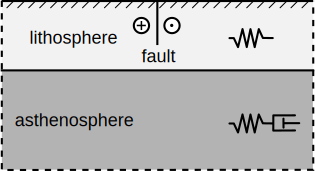
\includegraphics{schematic}
\caption
[Schematic of a postseismic deformation model]
{Schematic of a postseismic deformation model. A strike-slip fault is
embedded in an elastic layer which overlies a viscoelastic substrate.
This schematic is modeled after \citep{Savage1978}.}
\label{intro:fig:1}
\end{figure}

Some of the first observations of postseismic deformation came from
leveling and triangulation surveys \citep[e.g,][]{Kanamori1973,
Thatcher1975}. These geodetic techniques detected deformation to
within an accuracy of a few centimeters and at sampling intervals on
the order of years. 

\subsection{Slow Slip Events}

\section{Outline}
Chapter 2 presents a theoretical discussion on what can and cannot be
said about the strength of the lithosphere based on interseismic
deformation. Interseismic deformation is considered to be deformation
over the entire earthquake cycle (100s of years), whereas the
postseismic deformation mentioned above tends to refer to deformation
in the days to years following an earthquake. Both types of
deformation exhibit transients, although interseismic transients is
over a much longer timescale. Several studies have used interseismic
deformation to infer the strength of the crust and upper mantle. These
studies have almost unanimously concluded that the crust is relatively
strong compared to the upper mantle \citep{Thatcher2008}. In this
chapter I urge caution when interpreting the results of such studies,
because I demonstrate that their methodology is inherently biased
towards overestimating and underestimated the strength of the crust
and upper mantle, respectively. The bias results from the commonly
simplifying employed assumption that the viscosities are uniform
within the lower crust and upper mantle.

Chapter 3 and 4 focus on modeling postseismic deformation, where my
goal is to infer the lithospheric viscosity and distribution of
afterslip from observable postseismic deformation. Such an inverse
problem tends to be computationally intractable because there are many
unknown parameters being estimated. Additionally, the forward problem
is nonlinear with respect to the unknown parameters, and it must be
solved with numerical methods. In Chapter 3 we present a approximation
for the postseismic deformation forward problem that can be used to
make the inverse problem computationally tractable. We demonstrate
that our method is able to accurately identify the strength of the
lithospheric from postseismic deformation even while afterslip is
obscuring the signal from viscous relaxation. Chapter 4 is an
application of this method, where I analyze five years of postseismic
deformation following the 2010 El Mayor-Cucapah earthquake in Baja
California. One of my major findings in Chapter 4 is that an
accelerated rate of deformation can be observed several hundred
kilometers away for the earthquake epicenter. While this far reaching
deformation is not immediately recognizable from the raw GPS data, I
am able to observe a coherent signal after using a Kalman filtering
strategy that I developed and describe in this chapter. I then analyze
this postseismic signal to determine the physical mechanism causing
it. I find that the far field deformation is best described by a
Burgers rheology upper mantle with a transient viscosity of about
$10^{18}$ Pa$\cdot$s. My finding that the mantle is best described
with a Burgers rheology, rather than the more commonly employed
Maxwell rheology, is more consistent with mantle viscosities
determined in other types of geophysical studies
\citep[e.g.,][]{Crittenden1967,Bills1987}.

Chapter 5 is on quantifying noise in geodetic time series.  While this
chapter does not directly discuss transient deformation, it is
necessary to accurately quantify the noise in geodetic data before any
transient signal can be identified. We discuss a bias in a commonly
used method for quantifying noise in geodetic data. This bias tends to
underestimate the amplitude of noise, which then results in
underestimated uncertainties for any geophysical parameters derived
from the data. We demonstrate that the Restricted Maximum Likelihood
(REML) technique, which was first introduced by \citet{Patterson1971},
can be used as an alternative unbiased method for characterizing noise
in geodetic data.

In Chapter 6 we discuss a non-parametric method for detecting
transient deformation, specifically transient strain, in GNSS data.
Existing transient detection methods tend to assume a parametric form
for the underlying signal being detected \citep[e.g.,][]{Ohtani2010},
and an improperly chosen parameterization can bias the results. Our
method for detecting transient deformation uses Gaussian process
regression, where we assume a stochastic prior model for the
underlying signal. As opposed to a subjectively chosen parametric
model, our stochastic prior model can be objectively chosen using
maximum likelihood techniques, such as the REML method discussed in
Chapter 5. We demonstrate our method by applying it to GNSS data from
the Pacific Northwest, where we detect transient strain from slow slip
events. We verify the accuracy of our detection method by comparing
our inferred geophysical signal to observations of seismic tremor,
which are known to coincide with slow slip events.

Chapter 7 is a discussion on borehole strain meters (BSMs) and their
ability to record strain from slow slip events. The PBO contains 82
BSMs; however, the data recorded by these instruments is seldom used.
This is perhaps because it is unclear whether BSM data, which
describes strains over a 8.7 centimeter baseline, are representative
of regional tectonic strains. We address this question by comparing
GNSS derived strains, described in Chapter 6, to the strains recorded
at BSMs. We find that only two BSMs record data that is consistent
with the regional strains derived from GNSS data. A third station can
be made consistent with the GNSS derived strains if we assume that it
is misoriented.

Finally, in Chapter 8 we discuss future research directions and
provide concluding remarks.

\section{Publications from this dissertation}
This dissertation consists of three published manuscripts, two
manuscripts that are currently in review, and one manuscript that is
in preparation. The published and submitted manuscripts are listed
below.

\begin{itemize}
\item{Hines, T. T., and Hetland, E. A. (2013). Bias in estimates of lithosphere viscosity from interseismic deformation. Geophysical Research Letters, 40, 4260--4265, doi:10.1002/grl.50839. \textbf{Chapter 2}}  
\item{Hines, T. T., and Hetland, E. A. (2015). Rapid and simultaneous estimation of fault slip and heterogeneous lithospheric viscosity from post-seismic deformation. Geophysical Journal International, 204, 569–582, doi:10.1093/gji/ggv477. \textbf{Chapter 3}} 
\item{Hines, T. T., and Hetland, E. A. (2016). Rheologic constraints on the upper mantle from five years of postseismic deformation following the El Mayor-Cucapah earthquake. Journal of Geophysical Research: Solid Earth, 121, doi:10.1002/2016JB013114. \textbf{Chapter 4}}
\item{Hines, T. T., and Hetland, E. A. (2017). Unbiased characterization of noise in geodetic data. submitted to Journal of Geodesy \textbf{Chapter 5}}
\item{Hines, T. T., and Hetland, E. A. (2017). Revealing transient strain in geodetic data with Gaussian process regression. submitted to Geophysical Journal International \textbf{Chapter 6}} 
\end{itemize}
